\documentclass[a4paper,11pt,fontset=fandol]{article}
\usepackage{comment} % enables the use of multi-line comments (\ifx \fi)
\usepackage{lipsum} %This package just generates Lorem Ipsum filler text.
\usepackage{fullpage} % changes the margin
\usepackage{ctex}
\usepackage{ulem}
\usepackage{amsmath,amsthm,amssymb}
\usepackage{graphicx}
\usepackage{indentfirst}
\usepackage{caption}
\usepackage{hyperref}
\usepackage{subfigure}
\usepackage{float}
\usepackage{minted}


\renewcommand{\labelitemi}{$\blacksquare$}
\setcounter{secnumdepth}{3}
\setmonofont{Sarasa Mono SC}

\title{\heiti \texttt{C++}项目管理及工程实践\\ 分设计报告}
\author{毛文涵\quad 3170105380}
\date{\today}

\begin{document}
\maketitle

\section{分工任务及解决方案}
\subsection{分工任务}
本人负责Model层中矩阵类的实现,支持以下操作:
\begin{itemize}
  \item 打开图像文件
  \item 存储图像文件
  \item 获取图像尺寸
  \item 图像旋转
  \item 彩色图像灰度化、二值化
  \item 对比度、亮度调整
  \item 图像尺寸调整
  \item 图像人脸检测
  \item 卷积
  \item 获取及设置特定像素点
\end{itemize}

\subsection{解决方案}
\paragraph{架构说明} 项目整体采用MVVM架构,Model、ViewModel及View模块完全解耦,因此相关工作可在整体设计的基础上独立进行。

\paragraph{主要技术} 上述任务主要涉及用于表示图像的底层矩阵类及与用户交互的GUI界面,经分析后技术方案如下:
\begin{itemize}
  \item 底层矩阵类采用\texttt{OpenCV}计算机视觉库实现。
\end{itemize}

\section{设计思路}
\subsection{整体实现}
矩阵类负责处理底层图像的表示及相关操作处理,并为\texttt{Javascript}提供相关绑定。类的主要数据成员为一\texttt{cv::Mat}类型的矩阵,代表一张图片数据。每项操作(对比度及亮度调整、图像旋转等)较为整齐地对应两成员函数,其一负责图像本身的变换,另一函数实现其与\texttt{v8}的绑定,从而允许程序通过\texttt{Javascript}脚本对图像进行操作。

\subsection{主要细节}
\subsubsection{\texttt{v8}绑定}
借助\texttt{v8pp},我们可将\texttt{C++}类 、函数及变量等绑定至\texttt{v8},从而可直接由\texttt{Javascript}脚本对上述内容进行操作而无需手动编写解析程序。例如我们可将\texttt{Matrix}类及其成员函数\texttt{rotate}进行绑定,随后便可通过以下脚本
\begin{minted}{javascript}
    var mat = new Matrix();
    mat.rotate(60);
\end{minted}
实现等效于
\begin{minted}{c++}
    Matrix* mat = new Matrix();
    mat->rotate(60);
\end{minted}
的操作。此过程的目的并非以更简短的代码达到相同的功能,而是借助其自动生成的解释程序实现脚本运行,从而赋予程序批量处理、操作回溯等能力,这正是图形界面所欠缺的。

相关的绑定并不困难,示例代码如下:
\begin{minted}{c++}
  void DefineJSMatrix(V8Shell* shell) {
    if (gMatrixClass != nullptr) {
      return;
    }
    auto isolate = shell->GetIsolate();
    gMatrixClass = new v8pp::class_<Matrix>(isolate);
    (*gMatrixClass)
      .ctor <> ()
      // values
      .set("matrix", &Matrix::matrix)
      // functions
      .set("rotate", &Matrix::v8_rotate)
      .set("fill", &Matrix::fill)
      //...
      ;
  
    shell->RegisterClasses( {
        { "Matrix", (*gMatrixClass).js_function_template() }
      }
    );
  }
\end{minted}

其中\texttt{.set}部分将\texttt{Javascript}中的关键字与\texttt{C++}对象关联起来,其具体应用方式将于后文阐述。

\subsubsection{图像操作 - \texttt{Javascript}接口}
\texttt{Javascript}脚本(用户在命令行中输入的、由文件中读取的或程序运行过程中生成的)经解析后返回每条操作的参数\texttt{const v8::FunctionCallbackInfo<v8::Value>\& args}。仍以旋转图像的操作为例,下述代码

\begin{minted}{javascript}
    // var mat = new Matrix();
    mat.rotate(60);
\end{minted}
将返回\texttt{60}为参数。此只需将其转换为所需类型(此处为\texttt{double})即可获取用户输入的全部信息:
\begin{minted}{c++}
  double deg = v8pp::from_v8<double>(args.GetIsolate(), args[0], INT_MAX);
\end{minted}

此后以\texttt{deg}为参数调用相应函数即可完成操作:
\begin{minted}{c++}
    rotate(deg);
    return_this(args);
\end{minted}

此外,相关的错误处理是必要的:
\begin{minted}{c++}
    int num_args = args.Length();
    if (num_args == 0) {
      return ArgError(args, "Expected at least one argument");
    }
\end{minted}

\subsubsection{图像操作 - 底层处理}
由于图像操作种类较多但繁而不难,我们仅一例进行简要说明。

\paragraph{例:图像旋转}
旋转操作可由一旋转矩阵表征,因此需构建对应的旋转矩阵,这一过程视采取的策略而变化,我们选择在旋转后空余部分填充黑色像素点:
\begin{minted}{c++}
    cv::Mat moveImage(matrix.rows, matrix.cols, CV_8UC3, cv::Scalar(0, 0, 0));
    cv::Point2f center(matrix.cols/2, matrix.rows/2);
    cv::Mat M = getRotationMatrix2D(center, degree, 1);
    cv::warpAffine(matrix, moveImage, M, cv::Size(matrix.cols, matrix.rows));
\end{minted}

随后即可完成旋转操作:
\begin{minted}{c++}
    cv::circle(moveImage, center, 2, cv::Scalar(255,0,0));
    matrix = moveImage;
\end{minted}

其余操作类似,因而此处不再赘述。其中人脸识别功能使用了\texttt{OpenCV}库提供的相关模型。

\section{图表说明}
该类的大致结构如图\ref{1.1}所示,其中对称地展示了相关图像操作。
\begin{figure}[H]
    \centering
    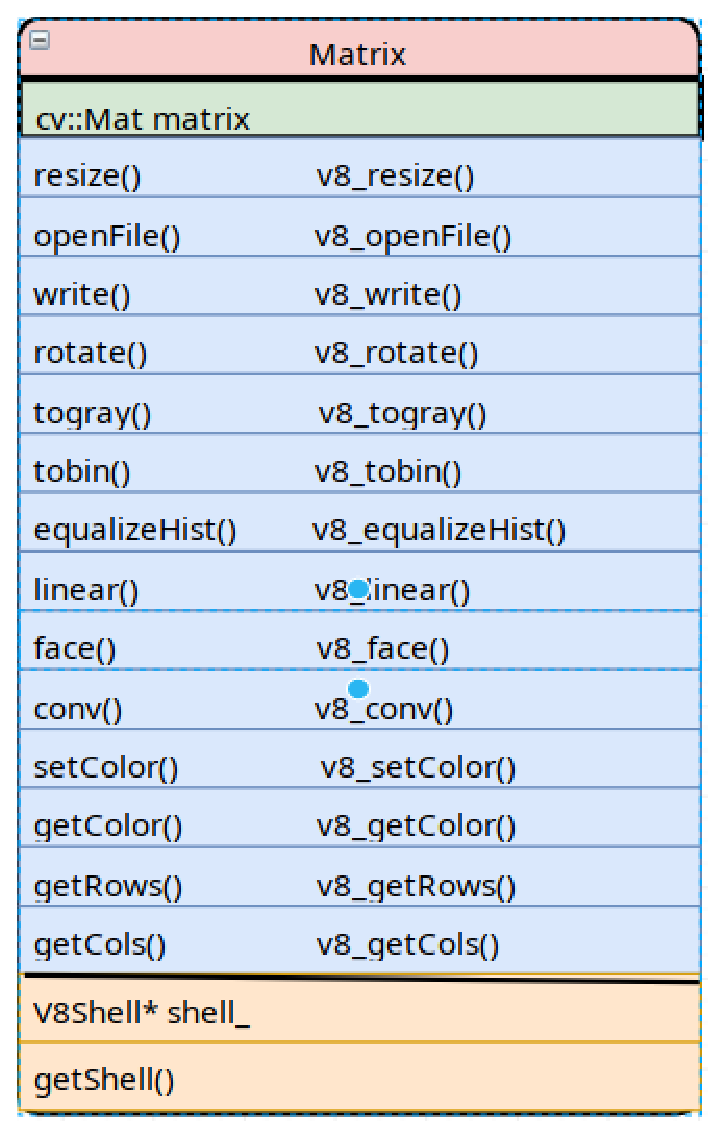
\includegraphics[scale=0.5]{fig//matrix.eps}
    \caption{\texttt{Matrix}类结构}
    \label{1.1}
\end{figure}

在此模块中,数据的流动及其与其他部分的联系如图\ref{1.2}所示。
\begin{figure}[H]
  \centering
  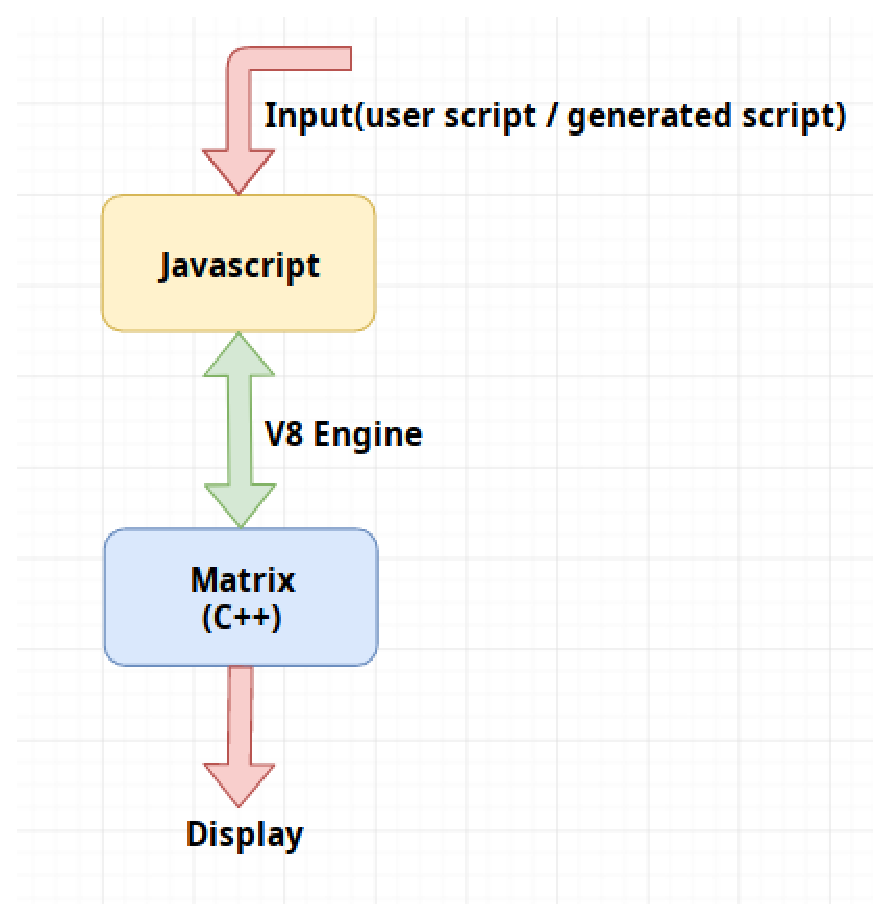
\includegraphics[scale=0.5]{fig//structure.eps}
  \caption{数据流动与模块关系}
  \label{1.2}
\end{figure}

\section{运行效果}
此模块不单独提供具有交互意义的运行结果,因此我们在此展示其与其他模块配合运作所得到的结果,其包括命令行模式及图形界面模式。

命令行模式对\texttt{Javascript}脚本进行解析并执行相应操作,其运行结果示例如图\ref{1.3}所示。
\begin{figure}[H]
  \centering
  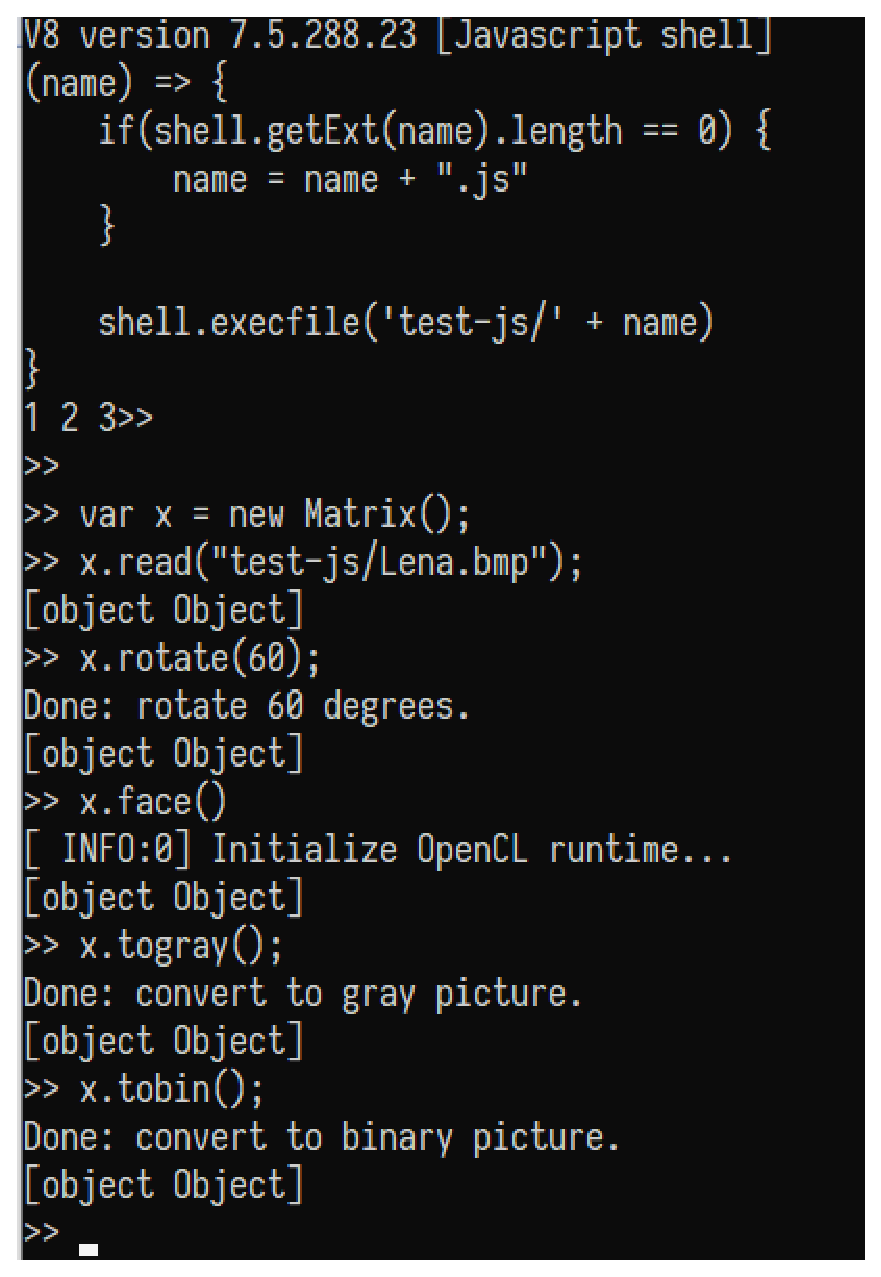
\includegraphics[scale=0.5]{fig//cli.eps}
  \caption{命令行模式运行结果}
  \label{1.3}
\end{figure}


图形界面模式下的交互是显然的,其运行结果示例如图\ref{1.4}所示。
\begin{figure}[H]
  \centering
  \subfigure[对比度调整]{
    \begin{minipage}{7cm}
      \centering
      \includegraphics[scale=0.2]{fig//gui1.eps}
    \end{minipage}
  }
  \subfigure[亮度调整及图像旋转]{
    \begin{minipage}{7cm}
      \centering
      \includegraphics[scale=0.2]{fig//gui2.eps}
    \end{minipage}
  }
  \subfigure[图像二值化]{
    \begin{minipage}{7cm}
      \centering
      \includegraphics[scale=0.2]{fig//gui3.eps}
    \end{minipage}
  }
  \subfigure[直方图均衡及人脸识别]{
    \begin{minipage}{7cm}
      \centering
      \includegraphics[scale=0.2]{fig//gui4.eps}
    \end{minipage}
  }
  \caption{图形模式运行结果}
  \label{1.4}
\end{figure}

\section{心得体会}
本项目具有较强的工程性质。使用现代开发工具与开发流程、按照低耦合度的MVVM架构进行设计开发的过程提升了将语言基本概念与方法投入到较为现代、贴近实际生产的工作中的能力。\texttt{Git}、\texttt{CI}等工具的使用提供了现代开发中最基础也是相当重要的辅助,这在以往非工程性质的课程中是难以接触到的。此外,开发过程也是对团队协作与交流能力的提升,亦可学到不少开发中不成文但重要的原则与规定。

\section{课程意见}
建议扩大选题范围,也即避免将图形界面作为主要的评价标准。事实上图形界面仅仅提高直观性与交互性的手段,其在某些情况下甚至是完全不需要的,尤其是编译/程序语言相关方面。

此外,作为一门工程性质的课程,十分有必要向\textbf{现代}工业界的部分标准、做法借鉴一二,而非墨守祖宗规矩。时代在进步,有些概念、方法即使不熟悉或下意识地不愿接受,也应以全面、客观的姿态看待,学术界及工业界对其的接受自然有其坚实的理论和实践积累,充耳不闻显然不是最好的做法。
\end{document}